\documentclass[12pt,arial]{article}
\usepackage[utf8]{inputenc}
\usepackage[brazil]{babel}
\usepackage{lipsum}
\usepackage{tabto}
\usepackage{graphicx}
\usepackage{graphics}
\usepackage{listings}

\hyphenation{palavra}
\usepackage[top=3cm,left=3cm,bottom=2cm,right=2cm]{geometry}
\usepackage{amsmath}

% Preencha com seu nome completo
\author{[SEU NOME COMPLETO]}
\usepackage{setspace}
\setstretch{1.5}
\begin{document}
	\begin{titlepage}
		\begin{center}
			\textbf{Universidade Federal de Viçosa}
			\textit{\\Campus}
			\textbf{Rio Paranaíba}
			\textnormal{\\\vspace{4cm}``[SEU NOME COMPLETO]'' - ``[SUA MATRÍCULA]"}
			\textbf{\\\vspace{5cm}``IMPLEMENTAÇÃO E ANÁLISE DOS ALGORITMOS INSERTION, SELECTION, BUBBLE E SHELL SORT"}
			\textbf{\\\vspace{9cm}Rio Paranaíba - MG \\ 2026}
		\end{center}
	\end{titlepage}

		\begin{titlepage}
			\begin{center}
				\textbf{Universidade Federal de Viçosa}
				\textit{\\Campus}
				\textbf{Rio Paranaíba}
				\textnormal{\\\vspace{3cm}``[SEU NOME COMPLETO]'' - ``[SUA MATRÍCULA]"}
				\textbf{\\\vspace{4cm}``IMPLEMENTAÇÃO E ANÁLISE DOS ALGORITMOS INSERTION, SELECTION, BUBBLE E SHELL SORT"\vspace{3cm}}
					\begin{flushright}
						\begin{minipage}{.5\textwidth}
							\textnormal{Trabalho apresentado para obtenção de créditos na disciplina de Projeto de Algoritmos da Universidade Federal de Viçosa - Campus de Rio Paranaíba.}
						\end{minipage}
					\end{flushright}

				\textbf{\\\vspace{3cm}Rio Paranaíba - MG \\ 2026}

			\end{center}
		\end{titlepage}


		\section{RESUMO}
		\qquad Este trabalho tem como objetivo implementar e analisar quatro
algoritmos clássicos de ordenação por comparação estudados na
disciplina de Projeto de Algoritmos: Insertion Sort, Selection Sort,
Bubble Sort e Shell Sort. Foi desenvolvida uma aplicação em C++,
com criação automática das pastas e arquivos pelo próprio programa,
capaz de gerar instâncias de teste de diferentes tamanhos (10, 100,
1.000, 10.000, 100.000 e 1.000.000 de elementos) e diferentes
características (crescente, decrescente e randômica), executar cada
algoritmo sobre elas e registrar o tempo de execução observado.

\qquad Os resultados foram organizados em arquivos de entrada, saída e
tempo para cada algoritmo, consolidados em tabelas e gráficos
individuais e comparativos que permitem analisar o comportamento de
cada algoritmo isoladamente e compará-los entre si. As medições
confirmam o comportamento teórico esperado para cada algoritmo:
desempenho linear no melhor caso do Insertion, Bubble e Shell Sort
(entrada já ordenada), desempenho quadrático constante em qualquer
caso para o Selection Sort, e uma clara superioridade prática do
Shell Sort sobre os demais algoritmos $O(n^2)$, evidenciando a forte
influência da estratégia de cada algoritmo — e, no caso do Insertion,
Selection e Bubble Sort, também do grau de ordenação inicial dos
dados — sobre o desempenho observado.

		\newpage

            % Sumário
		\tableofcontents
		\newpage

		\section{INTRODUÇÃO}
		\qquad Em várias situações do cotidiano é necessário manter conjuntos de
dados organizados: da lista telefônica ao histórico de transações
bancárias, a ordenação é uma operação central em ciência da
computação. Diante disso, diversos algoritmos de ordenação foram
desenvolvidos ao longo dos anos, cada um com características
próprias de desempenho, simplicidade de implementação e
comportamento em diferentes cenários de entrada.

\qquad Este trabalho é dividido em quatro capítulos, um para cada
algoritmo de ordenação estudado: o Capítulo 1 trata do Insertion
Sort, o Capítulo 2 do Selection Sort, o Capítulo 3 do Bubble Sort e
o Capítulo 4 do Shell Sort. Todos são algoritmos de ordenação por
comparação amplamente utilizados como introdução ao estudo de
algoritmos, e, com exceção do Shell Sort, todos possuem complexidade
$O(n^2)$ no pior caso — ainda que, dependendo dos dados de entrada,
alguns deles possam ser bem mais rápidos do que essa cota sugere.

\qquad Ao longo de cada capítulo são apresentados o funcionamento do
respectivo algoritmo, um teste de mesa manual, a análise de
complexidade nas diferentes situações de entrada, e os resultados
experimentais obtidos a partir de uma implementação em C++, testada
com instâncias de tamanhos crescentes (de 10 a 1.000.000 de
elementos) e três padrões de entrada: crescente, decrescente e
randômica. Ao final do trabalho, os quatro algoritmos são comparados
entre si por meio de uma tabela e um gráfico geral, seguidos de uma
conclusão consolidada sobre os resultados observados.

		\newpage

            \section{ALGORITMOS}
		\subsection{Insertion Sort}
		\qquad O Insertion Sort é um algoritmo de ordenação por comparação que
constrói a lista ordenada de forma incremental, um elemento por vez.
Sua lógica é semelhante à forma como uma pessoa organiza cartas de
baralho na mão: a cada nova carta recebida, ela é inserida na posição
correta em relação às cartas que já estão ordenadas.

\qquad O algoritmo percorre o vetor a partir do segundo elemento (índice 1).
A cada iteração, o elemento da posição atual, chamado de \textit{chave},
é comparado com os elementos anteriores, que já se encontram
ordenados entre si. Enquanto houver, à esquerda da chave, elementos
maiores que ela, esses elementos são deslocados uma posição à
frente, abrindo espaço para a chave ser inserida na posição correta.
Esse processo se repete até que todo o vetor tenha sido percorrido,
restando ao final um vetor completamente ordenado em ordem
crescente.

\qquad A seguir apresenta-se a implementação utilizada neste trabalho, em
C++, correspondente à função \texttt{InsertionSort\_versao1}:

\begin{verbatim}
void InsertionSort_versao1(int *vetor, int tamanho) {
    int chave, j;
    for (int i = 1; i < tamanho; i++) {
        chave = vetor[i];
        j = i - 1;
        while (j >= 0 && vetor[j] > chave) {
            vetor[j + 1] = vetor[j];
            j--;
        }
        vetor[j + 1] = chave;
    }
}
\end{verbatim}

\qquad Uma característica importante do Insertion Sort é que seu
desempenho depende diretamente do grau de ordenação da entrada:
quanto mais próxima a entrada já estiver da ordem final, menos
deslocamentos serão necessários durante a execução. Essa
característica é explorada em detalhes na análise de complexidade e
nos resultados experimentais apresentados nas próximas seções deste
capítulo.

\subsection{Teste de Mesa Manual}

\qquad Nesta seção deve ser inserida a digitalização do teste de mesa
manual do Insertion Sort, realizado à mão com um exemplo de entrada
diferente dos exemplos trabalhados em sala de aula, conforme exigido
pelo enunciado do trabalho. Substitua a imagem de exemplo abaixo pela
digitalização (foto ou escaneamento) do teste de mesa manuscrito.

\begin{figure}[htbp]
    \centering
    % Substitua o arquivo abaixo pela digitalizacao do teste de mesa manuscrito
    
\includegraphics[width=14cm]{Imagens/Insertion Sort/teste_de_mesa.png}
    \caption{Teste de mesa manual do algoritmo Insertion Sort}
    \label{fig:teste_mesa}
\end{figure}

		\newpage

		\subsection{Selection Sort}
		\qquad O Selection Sort é um algoritmo de ordenação por comparação baseado
na ideia de, repetidamente, selecionar o menor elemento ainda não
ordenado e colocá-lo em sua posição final. É um dos algoritmos mais
intuitivos: em vez de inserir elementos em uma sequência já ordenada
(como faz o Insertion Sort), o Selection Sort constrói a parte
ordenada do vetor da esquerda para a direita, sempre buscando, entre
os elementos restantes, aquele que deve ocupar a próxima posição.

\qquad O algoritmo percorre o vetor com um índice \textit{i}, de 0 até
tamanho-2. Para cada posição \textit{i}, é feita uma busca linear pelo
menor elemento entre as posições \textit{i} e tamanho-1. Encontrado o
menor elemento, ele é trocado de lugar com o elemento da posição
\textit{i} (a troca só é realizada se o menor encontrado não estiver
já na posição \textit{i}). Repetindo esse processo para todas as
posições, o vetor fica completamente ordenado em ordem crescente ao
final da execução.

\qquad A seguir apresenta-se a implementação utilizada neste trabalho, em
C++, correspondente à função \texttt{SelectionSort\_versao1}:

\begin{verbatim}
void SelectionSort_versao1(int *vetor, int tamanho) {
    int menor, aux;
    for (int i = 0; i < tamanho - 1; i++) {
        menor = i;
        for (int j = i + 1; j < tamanho; j++) {
            if (vetor[j] < vetor[menor]) {
                menor = j;
            }
        }
        if (menor != i) {
            aux = vetor[i];
            vetor[i] = vetor[menor];
            vetor[menor] = aux;
        }
    }
}
\end{verbatim}

\qquad Uma característica marcante do Selection Sort, explorada em detalhes
na análise de complexidade deste capítulo, é que o número de
\textit{comparações} realizadas não depende de a entrada já estar
ordenada, invertida ou embaralhada: a busca pelo menor elemento
sempre percorre integralmente os elementos restantes. Isso o
diferencia do Insertion Sort e do Bubble Sort, que se beneficiam de
entradas parcialmente ordenadas. A única grandeza que varia com o
tipo de entrada é o número de \textit{trocas}, que é, no máximo,
tamanho-1 em qualquer caso — uma quantidade desprezível diante do
número de comparações.

\subsection{Teste de Mesa Manual}

\qquad Nesta seção deve ser inserida a digitalização do teste de mesa
manual do Selection Sort, realizado à mão com um exemplo de entrada
diferente dos exemplos trabalhados em sala de aula, conforme exigido
pelo enunciado do trabalho. Substitua a imagem de exemplo abaixo pela
digitalização (foto ou escaneamento) do teste de mesa manuscrito.

\begin{figure}[htbp]
    \centering
    % Substitua o arquivo abaixo pela digitalizacao do teste de mesa manuscrito
    
\includegraphics[width=14cm]{Imagens/Selection Sort/teste_de_mesa.png}
    \caption{Teste de mesa manual do algoritmo Selection Sort}
    \label{fig:teste_mesa_selection}
\end{figure}

		\newpage

		\subsection{Bubble Sort}
		\qquad O Bubble Sort (ou "ordenação por bolha") é um algoritmo de ordenação
por comparação que percorre repetidamente o vetor, comparando pares de
elementos \textit{adjacentes} e trocando-os de posição sempre que
estiverem fora de ordem. A cada passada completa pelo vetor, o maior
elemento ainda não posicionado "borbulha" até a sua posição final, de
forma análoga a uma bolha de ar subindo até a superfície — daí o nome
do algoritmo.

\qquad O algoritmo realiza, no máximo, tamanho-1 passadas. Em cada passada
\textit{i}, percorre-se o vetor comparando os pares (vetor[j],
vetor[j+1]), trocando-os quando vetor[j] > vetor[j+1]. A versão
implementada neste trabalho inclui uma otimização amplamente utilizada
na prática: uma variável de controle (\textit{trocou}) que registra se
alguma troca ocorreu durante a passada. Caso nenhuma troca tenha
ocorrido, o vetor já está ordenado e o algoritmo é interrompido
imediatamente, sem realizar as passadas restantes — isso é o que
torna o comportamento do algoritmo linear quando a entrada já está
ordenada.

\qquad A seguir apresenta-se a implementação utilizada neste trabalho, em
C++, correspondente à função \texttt{BubbleSort\_versao1}:

\begin{verbatim}
void BubbleSort_versao1(int *vetor, int tamanho) {
    int aux;
    bool trocou;
    for (int i = 0; i < tamanho - 1; i++) {
        trocou = false;
        for (int j = 0; j < tamanho - 1 - i; j++) {
            if (vetor[j] > vetor[j + 1]) {
                aux = vetor[j];
                vetor[j] = vetor[j + 1];
                vetor[j + 1] = aux;
                trocou = true;
            }
        }
        if (!trocou) break;
    }
}
\end{verbatim}

\qquad Assim como o Insertion Sort, o Bubble Sort se beneficia de entradas
já ordenadas ou quase ordenadas, apresentando desempenho linear nesse
cenário graças à parada antecipada. Por outro lado, em entradas
decrescentes ou aleatórias, o algoritmo realiza um número de
comparações da mesma ordem de grandeza do Insertion Sort, porém com um
custo maior por troca (três atribuições contra uma no deslocamento do
Insertion Sort), o que costuma torná-lo mais lento na prática, como
discutido na análise de complexidade e evidenciado nos resultados
experimentais deste capítulo.

\subsection{Teste de Mesa Manual}

\qquad Nesta seção deve ser inserida a digitalização do teste de mesa
manual do Bubble Sort, realizado à mão com um exemplo de entrada
diferente dos exemplos trabalhados em sala de aula, conforme exigido
pelo enunciado do trabalho. Substitua a imagem de exemplo abaixo pela
digitalização (foto ou escaneamento) do teste de mesa manuscrito.

\begin{figure}[htbp]
    \centering
    % Substitua o arquivo abaixo pela digitalizacao do teste de mesa manuscrito
    
\includegraphics[width=14cm]{Imagens/Bubble Sort/teste_de_mesa.png}
    \caption{Teste de mesa manual do algoritmo Bubble Sort}
    \label{fig:teste_mesa_bubble}
\end{figure}

		\newpage

		\subsection{Shell Sort}
		\qquad O Shell Sort é um algoritmo de ordenação por comparação que pode ser
entendido como uma generalização do Insertion Sort. Em vez de comparar
e deslocar apenas elementos adjacentes desde o início, o Shell Sort
primeiro ordena, de forma aproximada, subconjuntos de elementos
espaçados por um intervalo (chamado de \textit{gap}), e vai reduzindo
progressivamente esse intervalo até chegar a 1 — quando o algoritmo se
comporta exatamente como um Insertion Sort tradicional, porém sobre um
vetor que já está quase ordenado, o que reduz drasticamente o número
de deslocamentos necessários nessa última etapa.

\qquad A implementação utilizada neste trabalho adota a sequência de
intervalos originalmente proposta por Donald Shell: o primeiro
intervalo é tamanho/2, e a cada passada o intervalo é dividido por 2
(divisão inteira), até chegar a 1. Para cada intervalo (gap), aplica-se
a lógica do Insertion Sort a cada um dos subvetores formados por
elementos espaçados de \textit{gap} posições entre si.

\qquad A seguir apresenta-se a implementação utilizada neste trabalho, em
C++, correspondente à função \texttt{ShellSort\_versao1}:

\begin{verbatim}
void ShellSort_versao1(int *vetor, int tamanho) {
    int chave, j;
    for (int gap = tamanho / 2; gap > 0; gap /= 2) {
        for (int i = gap; i < tamanho; i++) {
            chave = vetor[i];
            j = i - gap;
            while (j >= 0 && vetor[j] > chave) {
                vetor[j + gap] = vetor[j];
                j -= gap;
            }
            vetor[j + gap] = chave;
        }
    }
}
\end{verbatim}

\qquad A escolha da sequência de intervalos é um dos aspectos mais
estudados do Shell Sort, pois afeta diretamente sua complexidade de
pior caso — esse ponto é discutido em detalhes, com base em pesquisa
bibliográfica, na seção de análise de complexidade deste capítulo,
conforme solicitado no enunciado do trabalho. De forma geral, mesmo
utilizando a sequência mais simples (a original de Shell), o algoritmo
apresenta desempenho muito superior ao Insertion, Selection e Bubble
Sort na prática, para todos os tipos de entrada testados.

\subsection{Teste de Mesa Manual}

\qquad Nesta seção deve ser inserida a digitalização do teste de mesa
manual do Shell Sort, realizado à mão com um exemplo de entrada
diferente dos exemplos trabalhados em sala de aula, conforme exigido
pelo enunciado do trabalho. Substitua a imagem de exemplo abaixo pela
digitalização (foto ou escaneamento) do teste de mesa manuscrito.

\begin{figure}[htbp]
    \centering
    % Substitua o arquivo abaixo pela digitalizacao do teste de mesa manuscrito
    
\includegraphics[width=14cm]{Imagens/Shell Sort/teste_de_mesa.png}
    \caption{Teste de mesa manual do algoritmo Shell Sort}
    \label{fig:teste_mesa_shell}
\end{figure}

		\newpage

            \section{ANÁLISE DE COMPLEXIDADE}
		\subsection{Insertion Sort}
		\qquad A análise de complexidade do Insertion Sort, considerando as
diferentes situações de entrada (crescente, decrescente e
randômica), foi realizada manuscrita, com a devida justificativa,
conforme exigido pelo enunciado do trabalho. A digitalização do
material manuscrito deve ser inserida a seguir, substituindo a
imagem de exemplo abaixo.

\begin{figure}[htbp]
    \centering
    % Substitua o arquivo abaixo pela digitalizacao da analise de complexidade manuscrita
    \includegraphics[width=14cm]{Imagens/Insertion Sort/analise_complexidade.png}
    \caption{Análise de complexidade manuscrita do algoritmo Insertion Sort}
    \label{fig:analise_complexidade}
\end{figure}

\qquad Os resultados experimentais apresentados na próxima seção deste
capítulo são compatíveis com essa análise teórica: desempenho linear
no melhor caso (entrada crescente) e desempenho quadrático no caso
médio e no pior caso (entradas randômica e decrescente).

	    \newpage

		\subsection{Selection Sort}
		\qquad A análise de complexidade do Selection Sort, considerando as
diferentes situações de entrada (crescente, decrescente e
randômica), foi realizada manuscrita, com a devida justificativa,
conforme exigido pelo enunciado do trabalho. A digitalização do
material manuscrito deve ser inserida a seguir, substituindo a
imagem de exemplo abaixo.

\begin{figure}[htbp]
    \centering
    % Substitua o arquivo abaixo pela digitalizacao da analise de complexidade manuscrita
    \includegraphics[width=14cm]{Imagens/Selection Sort/analise_complexidade.png}
    \caption{Análise de complexidade manuscrita do algoritmo Selection Sort}
    \label{fig:analise_complexidade_selection}
\end{figure}

\qquad Diferentemente do Insertion Sort e do Bubble Sort, a análise mostra
que o número de comparações do Selection Sort não depende do tipo de
entrada: em todos os casos (melhor, médio e pior) o algoritmo realiza
n(n-1)/2 comparações, resultando em complexidade $\Theta(n^2)$ nos três
cenários. O que varia entre os cenários é apenas o número de trocas
(no máximo n-1), uma quantidade desprezível diante do número de
comparações. Os resultados experimentais apresentados na próxima
seção confirmam essa previsão teórica: os tempos medidos para entradas
crescente, decrescente e randômica são praticamente idênticos entre
si, para um mesmo tamanho de instância.

	    \newpage

		\subsection{Bubble Sort}
		\qquad A análise de complexidade do Bubble Sort, considerando as
diferentes situações de entrada (crescente, decrescente e
randômica), foi realizada manuscrita, com a devida justificativa,
conforme exigido pelo enunciado do trabalho. A digitalização do
material manuscrito deve ser inserida a seguir, substituindo a
imagem de exemplo abaixo.

\begin{figure}[htbp]
    \centering
    % Substitua o arquivo abaixo pela digitalizacao da analise de complexidade manuscrita
    \includegraphics[width=14cm]{Imagens/Bubble Sort/analise_complexidade.png}
    \caption{Análise de complexidade manuscrita do algoritmo Bubble Sort}
    \label{fig:analise_complexidade_bubble}
\end{figure}

\qquad Os resultados experimentais apresentados na próxima seção deste
capítulo são compatíveis com essa análise teórica: desempenho linear
no melhor caso (entrada crescente, graças à parada antecipada quando
nenhuma troca ocorre em uma passada) e desempenho quadrático no caso
médio e no pior caso (entradas randômica e decrescente). Vale destacar
que, apesar de Insertion Sort e Bubble Sort compartilharem a mesma
ordem de grandeza no pior caso, o Bubble Sort tende a ser mais lento
na prática, pois cada troca custa três atribuições, contra apenas uma
atribuição por deslocamento no Insertion Sort — o que também é
confirmado pelos tempos medidos.

	    \newpage

		\subsection{Shell Sort}
		\qquad Conforme orientado no enunciado do trabalho, a análise do Shell
Sort não segue o mesmo roteiro de contagem de instruções aplicado aos
demais algoritmos, pois sua complexidade depende diretamente da
sequência de intervalos (\textit{gaps}) utilizada. Em vez disso, foi
realizada uma pesquisa bibliográfica sobre a complexidade da sequência
de gaps efetivamente utilizada na implementação (a sequência original
de Shell: tamanho/2, tamanho/4, ..., 1), cujo conteúdo manuscrito deve
ser inserido a seguir, substituindo a imagem de exemplo abaixo.

\begin{figure}[htbp]
    \centering
    % Substitua o arquivo abaixo pela digitalizacao da pesquisa/analise manuscrita
    \includegraphics[width=14cm]{Imagens/Shell Sort/analise_complexidade.png}
    \caption{Pesquisa e análise de complexidade manuscrita do algoritmo Shell Sort}
    \label{fig:analise_complexidade_shell}
\end{figure}

\qquad Em resumo, a sequência de Shell utilizada tem pior caso teórico
$\Theta(n^2)$ (resultado devido a Donald Knuth), mas esse pior caso
exige uma disposição de dados especificamente construída para isso —
uma simples entrada decrescente não é suficiente para atingi-lo, pois
qualquer subsequência de um vetor decrescente também está em ordem
decrescente, o que mantém os deslocamentos de cada passada limitados.
Por isso, tanto a entrada crescente quanto a decrescente apresentaram,
nos testes deste trabalho, comportamento próximo de $O(n \log n)$,
enquanto a entrada randômica apresentou um comportamento empírico
intermediário, sem uma fórmula fechada simples de caso médio conhecida
na literatura para esta sequência específica de gaps. Ainda assim,
mesmo utilizando a sequência mais simples possível, o Shell Sort
superou folgadamente os demais algoritmos deste trabalho em todos os
tipos de entrada testados, como mostram os resultados da próxima
seção.

	    \newpage

		\section{TABELA E GRÁFICO}
            \subsection{Insertion Sort}
		\qquad A Tabela \ref{tab:tempos_insertion} apresenta os tempos de execução,
em segundos, obtidos para o Insertion Sort nos seis tamanhos de
instância exigidos pelo trabalho, para cada um dos três tipos de
entrada testados.

\begin{table}[htbp]
    \centering
    \begin{tabular}{|l|r|r|r|r|r|r|}
        \hline
         & 10 & 100 & 1.000 & 10.000 & 100.000 & 1.000.000 \\
        \hline
        Crescente & 0,000001 & 0,000002 & 0,000002 & 0,000016 & 0,000094 & 0,001015 \\
        \hline
        Decrescente & 0,000002 & 0,000003 & 0,000146 & 0,013730 & 1,378020 & 139,297525 \\
        \hline
        Random & 0,000001 & 0,000003 & 0,000076 & 0,007502 & 0,689424 & 69,702984 \\
        \hline
    \end{tabular}
    \caption{Tempo de execução (em segundos) do Insertion Sort por tamanho e tipo de instância}
    \label{tab:tempos_insertion}
\end{table}

\qquad O Gráfico \ref{fig:grafico_insert} apresenta esses mesmos dados em
escala linear. Nele fica evidente que, para tamanhos de até 10.000
elementos, os tempos de execução são praticamente imperceptíveis nas
três situações. A diferença de comportamento só se torna visualmente
clara a partir de 100.000 elementos, quando o tempo das entradas
decrescente e randômica cresce de forma acentuada, enquanto a
entrada crescente permanece próxima de zero.

\begin{figure}[htbp]
    \centering
    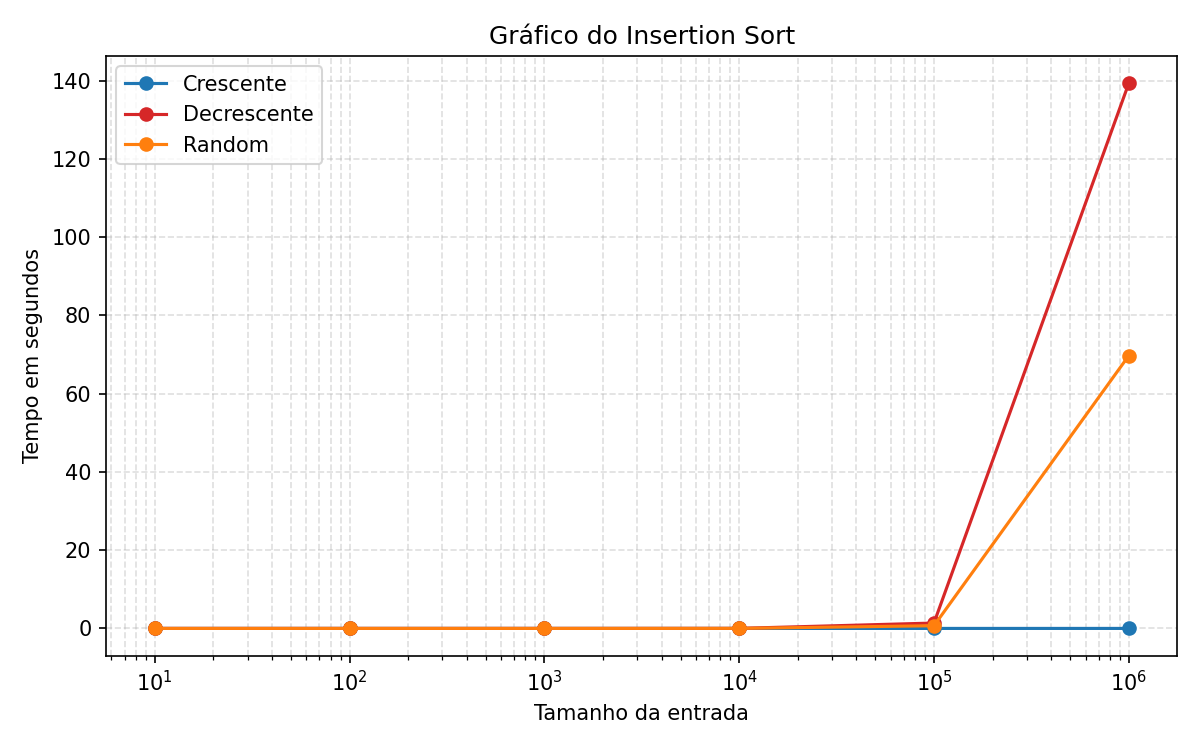
\includegraphics[width=14cm]{Imagens/Insertion Sort/grafico.png}
    \caption{Gráfico de tempo por tamanho do algoritmo Insertion Sort (escala linear)}
    \label{fig:grafico_insert}
\end{figure}

\qquad Como o crescimento quadrático faz com que os valores nas menores
instâncias fiquem visualmente esmagados no gráfico em escala linear,
o Gráfico \ref{fig:grafico_insert_log} apresenta os mesmos dados em
escala logarítmica no eixo do tempo, o que permite observar o
comportamento do algoritmo em todos os tamanhos testados, inclusive
os menores.

\begin{figure}[htbp]
    \centering
    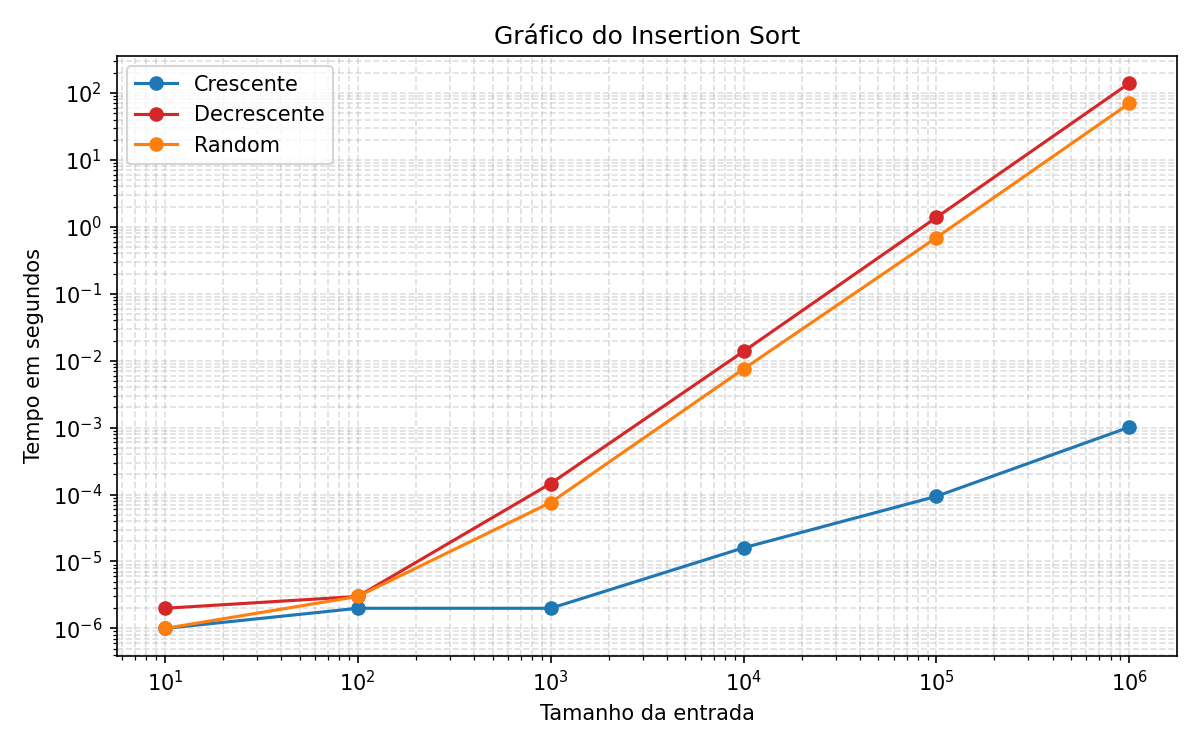
\includegraphics[width=14cm]{Imagens/Insertion Sort/grafico_log.png}
    \caption{Gráfico de tempo por tamanho do algoritmo Insertion Sort (escala logarítmica)}
    \label{fig:grafico_insert_log}
\end{figure}

\qquad Analisando os resultados, observa-se que a entrada crescente
apresenta desempenho linear: mesmo para 1.000.000 de elementos, o
tempo de execução foi de apenas cerca de 0,001 segundo, já que o
laço interno de deslocamento praticamente não é executado quando o
vetor já está ordenado. Já a entrada decrescente, que representa o
pior caso do algoritmo, teve o tempo de execução crescendo de forma
quadrática, chegando a aproximadamente 139,3 segundos para 1.000.000
de elementos. A entrada randômica, representando o caso médio,
também cresceu de forma quadrática, porém com tempo de execução
próximo à metade do pior caso (cerca de 69,7 segundos para 1.000.000
de elementos), o que é compatível com o número esperado de
comparações e deslocamentos em uma entrada aleatória.

		\newpage

		\subsection{Selection Sort}
		A Tabela \ref{tab:tempos_selection} apresenta os tempos de execução, em segundos, obtidos para o Selection Sort nos seis tamanhos de instância exigidos pelo trabalho, para cada um dos três tipos de entrada testados.

\begin{table}[htbp]
    \centering
    \begin{tabular}{|l|r|r|r|r|r|r|}
        \hline
         & 10 & 100 & 1.000 & 10.000 & 100.000 & 1.000.000 \\
        \hline
        Crescente & 0,000001 & 0,000008 & 0,001218 & 0,125560 & 12,468661 & 323,090207 \\
        \hline
        Decrescente & 0,000001 & 0,000010 & 0,001194 & 0,122701 & 12,588413 & 306,210246 \\
        \hline
        Random & 0,000001 & 0,000013 & 0,001230 & 0,116897 & 12,419415 & 321,875258 \\
        \hline
    \end{tabular}
    \caption{Tempo de execução (em segundos) do Selection Sort por tamanho e tipo de instância}
    \label{tab:tempos_selection}
\end{table}

O Gráfico \ref{fig:grafico_selection} apresenta esses mesmos dados em escala linear. Diferentemente do Insertion Sort, aqui as três curvas ficam praticamente sobrepostas em todos os tamanhos, o que já era esperado pela análise de complexidade: o número de comparações do Selection Sort não depende do tipo de entrada.

\begin{figure}[htbp]
    \centering
    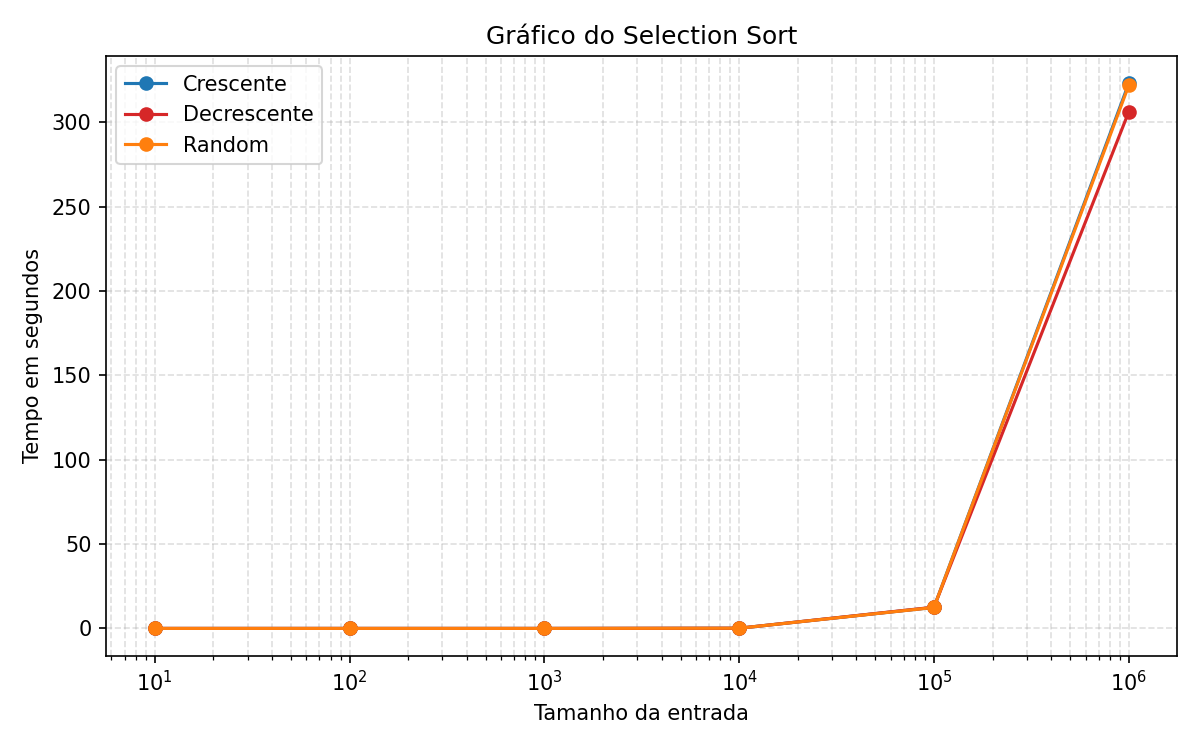
\includegraphics[width=14cm]{Imagens/Selection Sort/grafico.png}
    \caption{Gráfico de tempo por tamanho do algoritmo Selection Sort (escala linear)}
    \label{fig:grafico_selection}
\end{figure}

Como as três curvas são muito próximas, o Gráfico \ref{fig:grafico_selection_log} em escala logarítmica ajuda a confirmar que, mesmo em pequena escala, os tempos de Crescente, Decrescente e Random seguem lado a lado durante todo o intervalo de tamanhos testado -- a assinatura característica de um algoritmo cujo número de comparações independe da ordem dos dados de entrada, conforme discutido na análise de complexidade deste capítulo.

\begin{figure}[htbp]
    \centering
    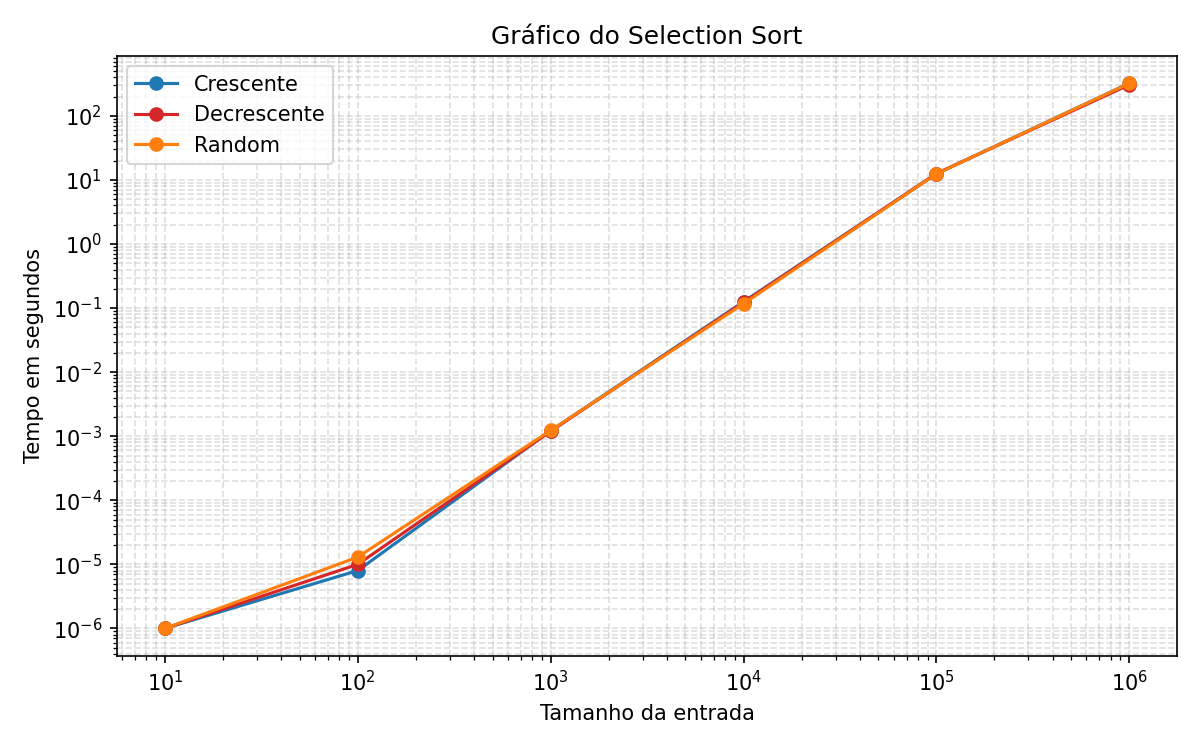
\includegraphics[width=14cm]{Imagens/Selection Sort/grafico_log.png}
    \caption{Gráfico de tempo por tamanho do algoritmo Selection Sort (escala logarítmica)}
    \label{fig:grafico_selection_log}
\end{figure}

		\newpage

		\subsection{Bubble Sort}
		A Tabela \ref{tab:tempos_bubble} apresenta os tempos de execução, em segundos, obtidos para o Bubble Sort nos seis tamanhos de instância exigidos pelo trabalho, para cada um dos três tipos de entrada testados.

\begin{table}[htbp]
    \centering
    \begin{tabular}{|l|r|r|r|r|r|r|}
        \hline
         & 10 & 100 & 1.000 & 10.000 & 100.000 & 1.000.000 \\
        \hline
        Crescente & 0,000001 & 0,000000 & 0,000001 & 0,000007 & 0,000091 & 0,001795 \\
        \hline
        Decrescente & 0,000000 & 0,000031 & 0,003800 & 0,320914 & 33,378878 & 3329,210083 \\
        \hline
        Random & 0,000001 & 0,000022 & 0,002098 & 0,179071 & 27,737162 & - \\
        \hline
    \end{tabular}
    \caption{Tempo de execução (em segundos) do Bubble Sort por tamanho e tipo de instância}
    \label{tab:tempos_bubble}
\end{table}

O Gráfico \ref{fig:grafico_bubble} apresenta esses mesmos dados em escala linear. Assim como no Insertion Sort, a entrada crescente permanece praticamente em zero em todos os tamanhos (graças à parada antecipada do algoritmo), enquanto as entradas decrescente e randômica crescem de forma acentuada a partir de 10.000 elementos.

\begin{figure}[htbp]
    \centering
    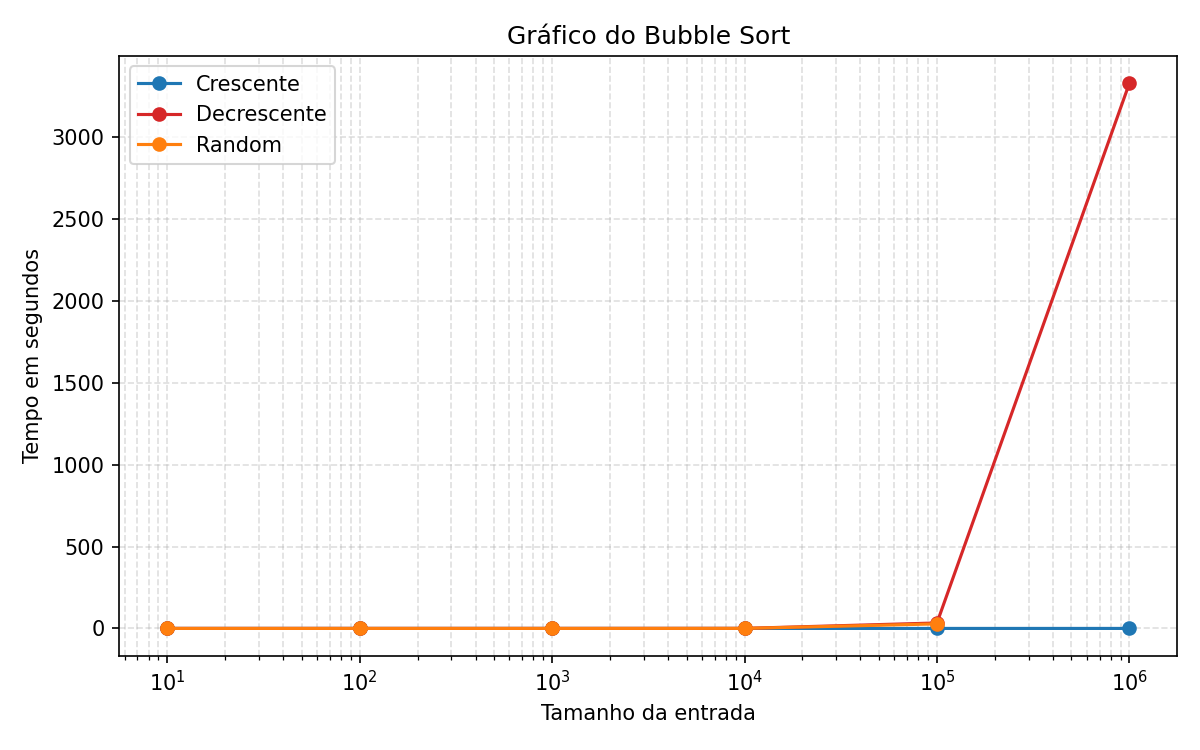
\includegraphics[width=14cm]{Imagens/Bubble Sort/grafico.png}
    \caption{Gráfico de tempo por tamanho do algoritmo Bubble Sort (escala linear)}
    \label{fig:grafico_bubble}
\end{figure}

O Gráfico \ref{fig:grafico_bubble_log} em escala logarítmica confirma o comportamento linear da entrada crescente e o comportamento quadrático das entradas decrescente e randômica. Comparando com o Insertion Sort (Capítulo 1), nota-se que o Bubble Sort é consistentemente mais lento nos casos decrescente e randômico, apesar de ambos terem a mesma ordem de grandeza de comparações -- diferença explicada pelo maior custo de cada troca do Bubble Sort (três atribuições) em comparação com o deslocamento do Insertion Sort (uma atribuição), como discutido na análise de complexidade.

\begin{figure}[htbp]
    \centering
    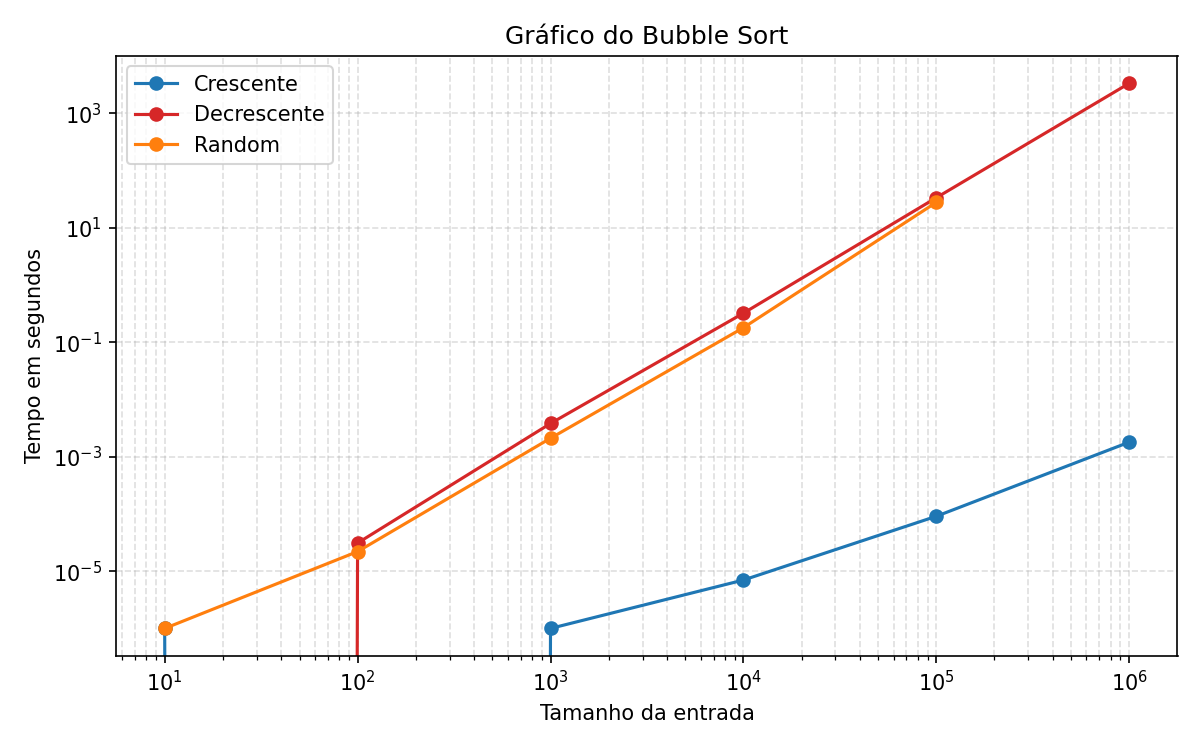
\includegraphics[width=14cm]{Imagens/Bubble Sort/grafico_log.png}
    \caption{Gráfico de tempo por tamanho do algoritmo Bubble Sort (escala logarítmica)}
    \label{fig:grafico_bubble_log}
\end{figure}

		\newpage

		\subsection{Shell Sort}
		A Tabela \ref{tab:tempos_shell} apresenta os tempos de execução, em segundos, obtidos para o Shell Sort nos seis tamanhos de instância exigidos pelo trabalho, para cada um dos três tipos de entrada testados.

\begin{table}[htbp]
    \centering
    \begin{tabular}{|l|r|r|r|r|r|r|}
        \hline
         & 10 & 100 & 1.000 & 10.000 & 100.000 & 1.000.000 \\
        \hline
        Crescente & 0,000001 & 0,000001 & 0,000012 & 0,000081 & 0,001082 & 0,017349 \\
        \hline
        Decrescente & 0,000001 & 0,000002 & 0,000012 & 0,000134 & 0,001697 & 0,023871 \\
        \hline
        Random & 0,000001 & 0,000003 & 0,000066 & 0,000821 & 0,011081 & 0,169964 \\
        \hline
    \end{tabular}
    \caption{Tempo de execução (em segundos) do Shell Sort por tamanho e tipo de instância}
    \label{tab:tempos_shell}
\end{table}

O Gráfico \ref{fig:grafico_shell} apresenta esses mesmos dados em escala linear. Diferentemente dos três algoritmos anteriores, mesmo a entrada decrescente permanece com tempo de execução muito baixo -- como discutido na análise de complexidade, uma entrada totalmente decrescente não é o pior caso teórico da sequência de gaps utilizada.

\begin{figure}[htbp]
    \centering
    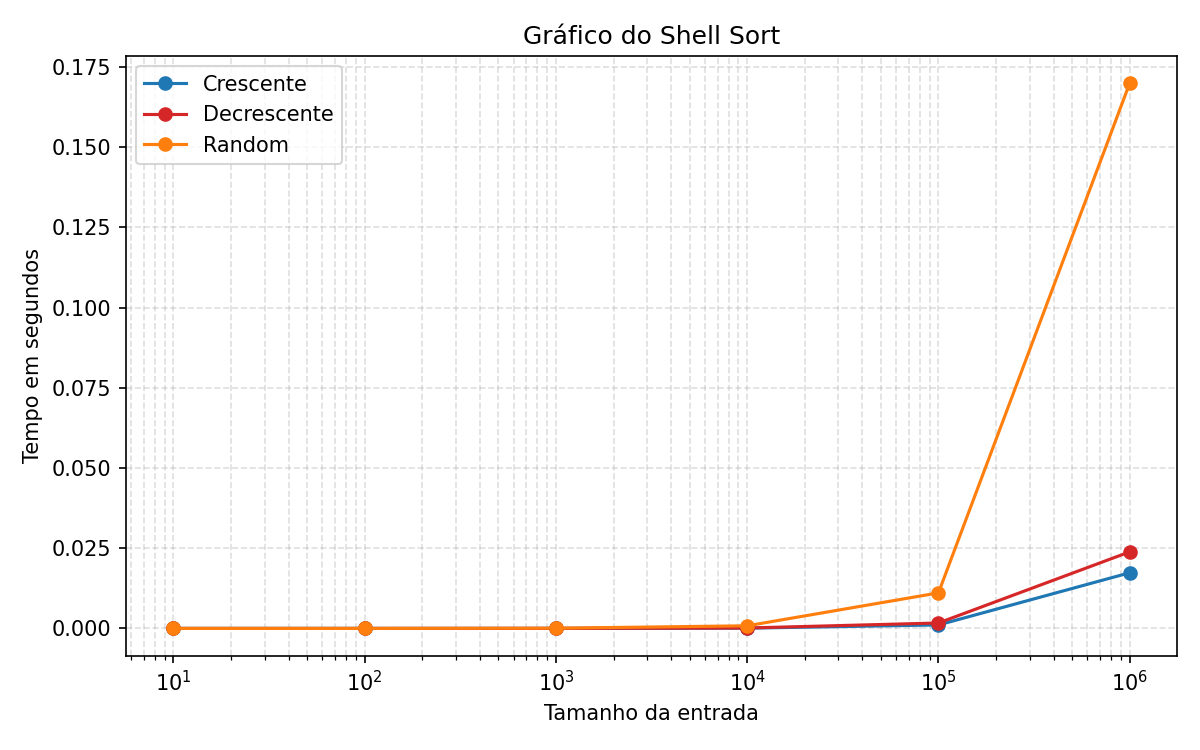
\includegraphics[width=14cm]{Imagens/Shell Sort/grafico.png}
    \caption{Gráfico de tempo por tamanho do algoritmo Shell Sort (escala linear)}
    \label{fig:grafico_shell}
\end{figure}

O Gráfico \ref{fig:grafico_shell_log} em escala logarítmica evidencia que mesmo a entrada randômica, a mais lenta das três para este algoritmo, é ordens de grandeza mais rápida do que qualquer um dos três algoritmos anteriores ($O(n^2)$) para o mesmo tamanho de instância -- a principal conclusão prática deste capítulo, retomada na Tabela de Comparação e no Gráfico Geral ao final deste trabalho.

\begin{figure}[htbp]
    \centering
    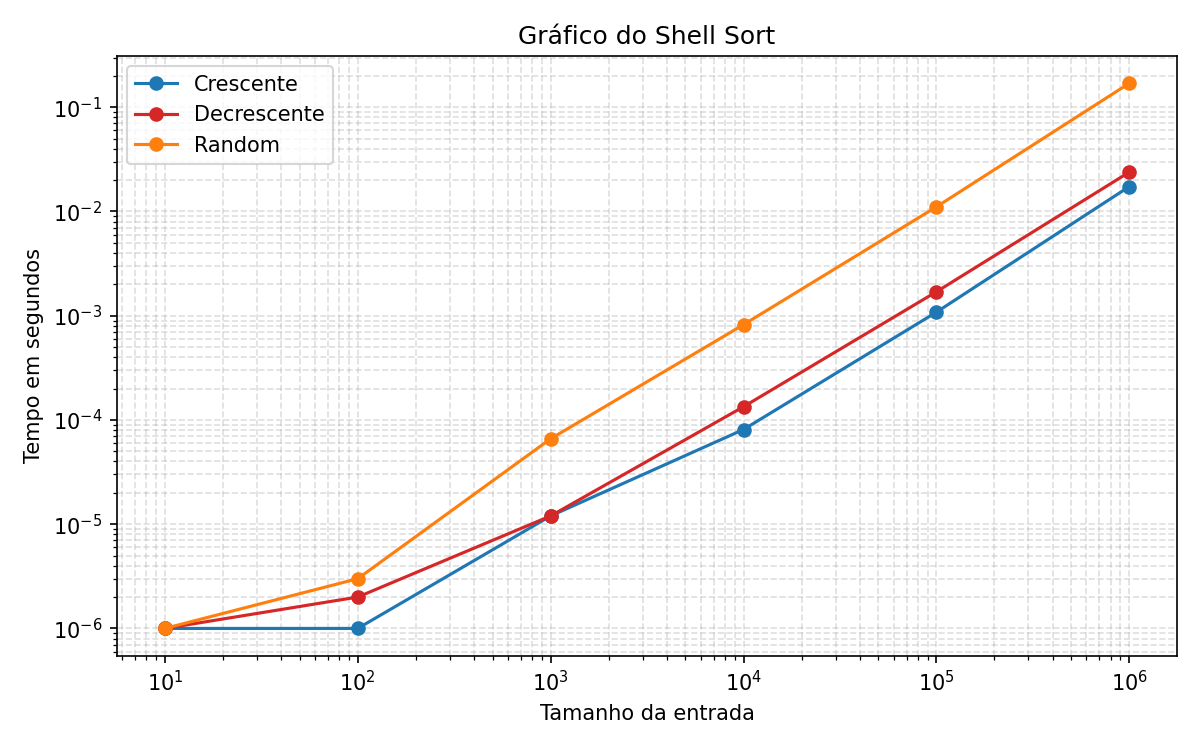
\includegraphics[width=14cm]{Imagens/Shell Sort/grafico_log.png}
    \caption{Gráfico de tempo por tamanho do algoritmo Shell Sort (escala logarítmica)}
    \label{fig:grafico_shell_log}
\end{figure}

		\newpage

		\section{TABELA DE COMPARAÇÃO}
		\qquad As Tabelas \ref{tab:comparacao_crescente}, \ref{tab:comparacao_decrescente}
e \ref{tab:comparacao_random} apresentam, lado a lado, os tempos de
execução (em segundos) obtidos pelos quatro algoritmos estudados neste
trabalho, para os seis tamanhos de instância exigidos, uma tabela para
cada um dos três tipos de entrada testados (Crescente, Decrescente e
Random).

\begin{table}[htbp]
    \centering
    \begin{tabular}{|l|r|r|r|r|r|r|}
        \hline
         & 10 & 100 & 1.000 & 10.000 & 100.000 & 1.000.000 \\
        \hline
        Insertion Sort & 0,000001 & 0,000002 & 0,000002 & 0,000016 & 0,000094 & 0,001015 \\
        \hline
        Selection Sort & 0,000001 & 0,000008 & 0,001218 & 0,125560 & 12,468661 & 323,090207 \\
        \hline
        Bubble Sort & 0,000001 & 0,000000 & 0,000001 & 0,000007 & 0,000091 & 0,001795 \\
        \hline
        Shell Sort & 0,000001 & 0,000001 & 0,000012 & 0,000081 & 0,001082 & 0,017349 \\
        \hline
    \end{tabular}
    \caption{Tempo de execução (em segundos) dos 4 algoritmos -- entrada Crescente}
    \label{tab:comparacao_crescente}
\end{table}

\begin{table}[htbp]
    \centering
    \begin{tabular}{|l|r|r|r|r|r|r|}
        \hline
         & 10 & 100 & 1.000 & 10.000 & 100.000 & 1.000.000 \\
        \hline
        Insertion Sort & 0,000002 & 0,000003 & 0,000146 & 0,013730 & 1,378020 & 139,297525 \\
        \hline
        Selection Sort & 0,000001 & 0,000010 & 0,001194 & 0,122701 & 12,588413 & 306,210246 \\
        \hline
        Bubble Sort & 0,000000 & 0,000031 & 0,003800 & 0,320914 & 33,378878 & 3329,210083 \\
        \hline
        Shell Sort & 0,000001 & 0,000002 & 0,000012 & 0,000134 & 0,001697 & 0,023871 \\
        \hline
    \end{tabular}
    \caption{Tempo de execução (em segundos) dos 4 algoritmos -- entrada Decrescente}
    \label{tab:comparacao_decrescente}
\end{table}

\begin{table}[htbp]
    \centering
    \begin{tabular}{|l|r|r|r|r|r|r|}
        \hline
         & 10 & 100 & 1.000 & 10.000 & 100.000 & 1.000.000 \\
        \hline
        Insertion Sort & 0,000001 & 0,000003 & 0,000076 & 0,007502 & 0,689424 & 69,702984 \\
        \hline
        Selection Sort & 0,000001 & 0,000013 & 0,001230 & 0,116897 & 12,419415 & 321,875258 \\
        \hline
        Bubble Sort & 0,000001 & 0,000022 & 0,002098 & 0,179071 & 27,737162 & - \\
        \hline
        Shell Sort & 0,000001 & 0,000003 & 0,000066 & 0,000821 & 0,011081 & 0,169964 \\
        \hline
    \end{tabular}
    \caption{Tempo de execução (em segundos) dos 4 algoritmos -- entrada Random}
    \label{tab:comparacao_random}
\end{table}


		\newpage

		\section{GRÁFICO GERAL}
		\qquad Os Gráficos \ref{fig:geral_crescente} e \ref{fig:geral_decrescente}
apresentam, respectivamente, o tempo de execução dos quatro algoritmos
estudados neste trabalho para entradas já ordenadas (crescente) e para
entradas em ordem decrescente (o cenário mais desfavorável para três dos
quatro algoritmos), permitindo comparar diretamente o desempenho de
Insertion Sort, Selection Sort, Bubble Sort e Shell Sort.

\begin{figure}[htbp]
    \centering
    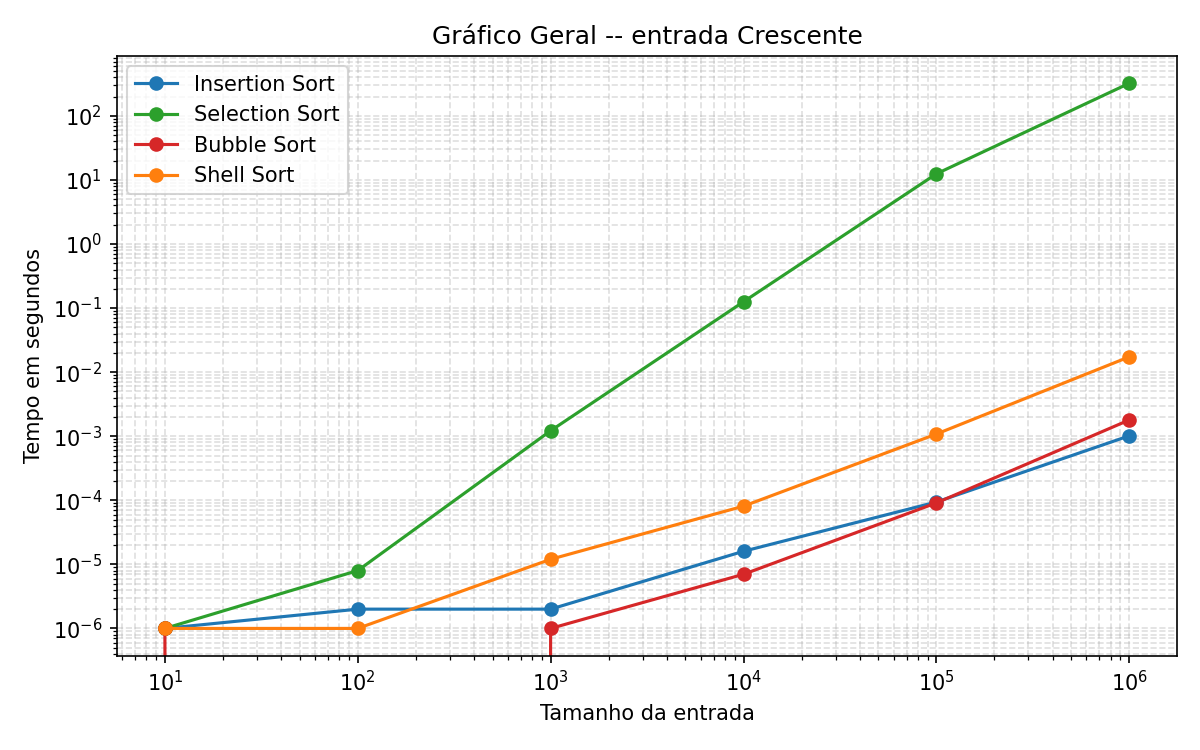
\includegraphics[width=14cm]{Imagens/Geral/grafico_geral_crescente_log.png}
    \caption{Gráfico geral (escala logarítmica) -- entrada crescente}
    \label{fig:geral_crescente}
\end{figure}

\begin{figure}[htbp]
    \centering
    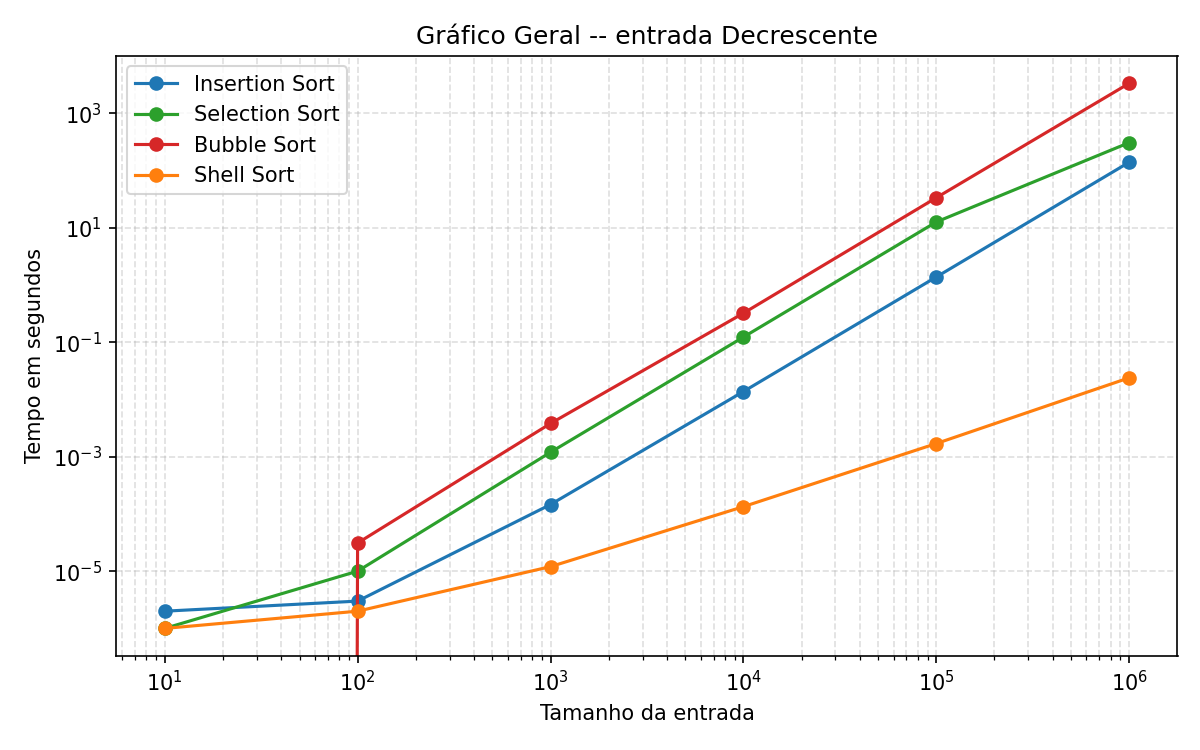
\includegraphics[width=14cm]{Imagens/Geral/grafico_geral_decrescente_log.png}
    \caption{Gráfico geral (escala logarítmica) -- entrada decrescente}
    \label{fig:geral_decrescente}
\end{figure}

		\newpage

		\section{CONCLUSÃO}
		\qquad A partir da implementação e dos experimentos realizados com os
quatro algoritmos, foi possível observar, na prática, diferenças de
comportamento que confirmam a análise teórica de cada um.

\qquad O \textbf{Insertion Sort} e o \textbf{Bubble Sort} compartilham uma
característica importante: ambos são sensíveis ao grau de ordenação
da entrada, apresentando desempenho linear ($O(n)$) quando os dados já
estão ordenados (entrada crescente) e desempenho quadrático ($O(n^2)$)
nos casos médio e pior (entradas randômica e decrescente,
respectivamente). Entre os dois, o Bubble Sort mostrou-se
consistentemente mais lento que o Insertion Sort para os mesmos
tamanhos e tipos de entrada, apesar de ambos terem a mesma ordem de
grandeza de comparações no pior e no caso médio — diferença
explicada pelo maior custo de cada troca do Bubble Sort (três
atribuições) frente ao deslocamento único do Insertion Sort.

\qquad O \textbf{Selection Sort} se destacou por um comportamento distinto:
sua complexidade é $\Theta(n^2)$ em \textit{todos} os casos (melhor, médio e
pior), já que o número de comparações não depende da ordem dos dados
de entrada — apenas o número de trocas varia, mas essa quantidade é
sempre $O(n)$ e, portanto, irrelevante diante das $O(n^2)$ comparações.
Isso foi confirmado experimentalmente: os tempos medidos para as
entradas crescente, decrescente e randômica ficaram praticamente
idênticos entre si, para um mesmo tamanho de instância.

\qquad O \textbf{Shell Sort} apresentou, de longe, o melhor desempenho entre
os quatro algoritmos, para todos os tipos de entrada testados, mesmo
utilizando a sequência de intervalos mais simples (a original de
Shell). Embora essa sequência tenha pior caso teórico $\Theta(n^2)$, esse
pior caso exige uma disposição de dados especificamente construída
para isso, o que não ocorre nem mesmo com uma entrada totalmente
decrescente — por isso, tanto a entrada crescente quanto a
decrescente exibiram comportamento próximo de O(n log n) nos testes
realizados, enquanto a entrada randômica, embora sem uma fórmula
fechada simples de caso médio, também se manteve ordens de grandeza
mais rápida que os demais algoritmos para os mesmos tamanhos.

\qquad Em resumo, os experimentos evidenciam que, embora Insertion,
Selection e Bubble Sort compartilhem a mesma complexidade assintótica
de pior caso ($O(n^2)$), a escolha entre eles pode fazer diferença
prática relevante dependendo do grau de ordenação esperado dos dados:
o Insertion Sort é preferível quando há expectativa de entradas quase
ordenadas, o Selection Sort tem a vantagem de um número previsível e
mínimo de trocas (útil quando a operação de escrita é cara), e o
Bubble Sort, apesar de didático, não apresenta vantagem prática clara
sobre os demais nos cenários testados. O Shell Sort, por sua vez,
demonstra como uma modificação relativamente simples do Insertion
Sort (a introdução de saltos/gaps decrescentes) é suficiente para
alcançar um ganho de desempenho expressivo, sendo a escolha mais
adequada dentre os quatro para instâncias grandes, especialmente
quando não é garantida nenhuma característica sobre a ordenação
prévia dos dados.

		\newpage

		\section{REFERÊNCIAS BIBLIOGRÁFICAS}
		CORMEN, Thomas H.; LEISERSON, Charles E.; RIVEST, Ronald L.; STEIN,
Clifford. \textit{Introduction to Algorithms}. 3. ed. Cambridge:
MIT Press, 2009.

SEDGEWICK, Robert; WAYNE, Kevin. \textit{Algorithms}. 4. ed.
Boston: Addison-Wesley, 2011.

KNUTH, Donald E. \textit{The Art of Computer Programming, Volume 3:
Sorting and Searching}. 2. ed. Boston: Addison-Wesley, 1998.

SHELL, Donald L. A High-Speed Sorting Procedure. \textit{Communications
of the ACM}, v. 2, n. 7, p. 30–32, 1959.


            % Não é necessário citar
		\section{Função para calcular o tempo}
		\qquad A seguir apresenta-se a função responsável por orquestrar, para
cada instância, a geração do vetor, a execução do algoritmo de
ordenação selecionado (recebido como um ponteiro de função, o que
permite reutilizar a mesma rotina para os quatro algoritmos deste
trabalho) com a respectiva medição de tempo, e o registro dos
arquivos de entrada, saída e tempo dentro da pasta correspondente ao
algoritmo — pasta essa que também é criada automaticamente pelo
próprio programa, caso ainda não exista (arquivos
\texttt{base.h} e \texttt{main.cpp}):

\begin{verbatim}
void criarEstruturaPastas(const string &algoritmo) {
    const string grupos[3] = {"Arquivos de Entrada", "Arquivos de Saida",
                               "Arquivos de Tempo"};
    const string categorias[3] = {"Crescente", "Decrescente", "Random"};
    for (const string &grupo : grupos)
        for (const string &categoria : categorias)
            fs::create_directories(algoritmo + "/" + grupo + "/" + categoria);
}

void operacoes(const string &algoritmo, FuncaoOrdenacao funcao,
               int tipo, int tamanho) {
    criarEstruturaPastas(algoritmo);

    clock_t start_t, end_t;
    double tempoGasto;

    int *vetor = gerarSequencia(tipo, tamanho);
    salvarEntrada(algoritmo, tipo, tamanho, vetor);

    start_t = clock();
    funcao(vetor, tamanho);
    end_t = clock();

    tempoGasto = (end_t - start_t) / (double)CLOCKS_PER_SEC;

    salvarTempo(algoritmo, tipo, tamanho, tempoGasto);
    salvarSaida(algoritmo, tipo, tamanho, vetor);

    delete[] vetor;
}
\end{verbatim}

\end{document}
